% =====================================================================
%  TELFOR 2026 -- Telecommunications Forum, Belgrade, Serbia
%  Paper: On HTAP Storage Configurations in SQL Server 2022:
%         An Empirical Evaluation
%  Authors: Nejra Smajlovic (University of Zenica, Polytechnic Faculty)
%           Alen Begovic (University of Sarajevo, Faculty of Electrical Eng.)
%
%  FORMAT COMPLIANCE (TELFOR instructions for authors):
%    * double-column A4, standard IEEE conference template (IEEEtran, 10 pt)
%    * maximum 4 A4 pages for regular and student papers
%    * submitted as PDF through the TELFOR online submission system
%
%  Build:  pdflatex telfor2026_htap.tex   (run twice)
% =====================================================================
\documentclass[10pt,conference,a4paper]{IEEEtran}
\IEEEoverridecommandlockouts

\usepackage[T1]{fontenc}
\usepackage[utf8]{inputenc}
\usepackage{cite}
\usepackage{graphicx}
\usepackage{amsmath}
\usepackage{booktabs}
\usepackage{balance}
\usepackage{url}
\usepackage[hidelinks]{hyperref}
\usepackage{upgreek}   % uspravna grcka slova: IEEE ne kurzivira grcke simbole

% --- Table typography -------------------------------------------------
\newcommand{\best}[1]{\textbf{#1}}

% --- Copyright notice at the bottom of the first page ------------------
% TELFOR's Instructions for Authors do not ask for an IEEE copyright line on
% the submitted paper, and the official IEEE conference template does not
% contain one, so the paper is submitted without it rather than with a
% placeholder ISBN. If TELFOR later publishes a copyright string for the
% camera-ready version, uncomment the three lines below and paste it in.
%\IEEEpubid{\parbox{\columnwidth}{\footnotesize
%  978-1-XXXX-XXXX-X/26/\$31.00~\copyright2026 IEEE\hfill}
%  \hspace{\columnsep}\makebox[\columnwidth]{}}

\begin{document}

\title{On HTAP Storage Configurations in SQL\\
Server 2022: An Empirical Evaluation}

\author{\IEEEauthorblockN{Nejra Smajlovi\'c}
\IEEEauthorblockA{\textit{University of Zenica}\\
\textit{Polytechnic Faculty}\\
Zenica, Bosnia and Herzegovina\\
nejra.smajlovic.22@size.ba}
\and
\IEEEauthorblockN{Alen Begovi\'c}
\IEEEauthorblockA{\textit{University of Sarajevo}\\
\textit{Faculty of Electrical Engineering}\\
Sarajevo, Bosnia and Herzegovina\\
alen.begovic@etf.unsa.ba}%
\thanks{N. Smajlovi\'c is with the Polytechnic Faculty, University of Zenica,
and A. Begovi\'c with the Faculty of Electrical Engineering, University of
Sarajevo, Bosnia and Herzegovina. Benchmark code, SQL scripts and
measurements: \url{https://github.com/itsnejra/htap-sqlserver-benchmark}.}}

\maketitle
\bstctlcite{bstctl:htap}

\begin{abstract}
This paper reports an independent empirical evaluation of four storage
configuration strategies available inside a single Microsoft SQL Server 2022
instance, for systems that must serve transactional and analytical queries
over the same data without the staleness and operational complexity of an
ETL-bridged data warehouse: disk-based tables with B-tree indexes
(Baseline), disk-based tables with a nonclustered columnstore index (CS),
memory-optimized tables on the Hekaton engine (IM), and a dual-store hybrid
configuration combining a memory-optimized transactional layer with a
columnstore analytical layer (HTAP). The experiment is a full factorial
design over four configurations, three OLTP/OLAP mixes and three concurrency
levels, with 30 repetitions per cell on the StackOverflow2010 dataset of
about 19.2 million rows per schema; 1,070 valid runs were analyzed with the
Kruskal-Wallis H test, Mann-Whitney U tests with Bonferroni correction,
Cohen's d and log-linear OLS regression. The dual-store configuration
dominates every tested scenario: it delivers 3.3 to 6.9 times the OLTP
throughput of the purely memory-optimized configuration under a
transaction-heavy mix and cuts median analytical latency by a factor of four
relative to the baseline. Because it separates
the two layers without paying any synchronization cost during measurement,
the reported gains represent an upper bound of the approach.
\end{abstract}

\begin{IEEEkeywords}
HTAP, In-Memory OLTP, columnstore index, SQL Server 2022, database
benchmarking, performance isolation.
\end{IEEEkeywords}

% =====================================================================
\section{Introduction}
% =====================================================================
\IEEEPARstart{M}{odern} information systems must serve two workload classes
with opposing requirements. Online transaction processing (OLTP) consists of
short atomic operations over individual records at high concurrency, under
strict consistency guarantees; online analytical processing (OLAP) relies on
long-running queries that aggregate millions of rows and demand high read
bandwidth. For three decades the standard answer to this tension has been
architectural separation: an operational database bridged to a data
warehouse by an extract-transform-load (ETL) pipeline whose delay is measured in
hours or days.
Hybrid transactional/analytical processing (HTAP), a term introduced by
Gartner in 2014, denotes the class of systems that aims to eliminate that
intermediary~\cite{ozcan2017}.

Microsoft SQL Server 2022 provides two built-in mechanisms for this purpose:
the Hekaton in-memory OLTP engine~\cite{diaconu2013} and columnstore
indexes~\cite{larson2013}. How they should be combined under mixed workloads
has not been systematically evaluated outside the vendor's own publications:
available HTAP benchmarking studies target distributed NewSQL systems or
rely on synthetic datasets (TPC-C, TPC-H) whose uniform access distributions
do not reproduce the Pareto-shaped activity of real web
applications~\cite{zhang2024hybench}.

This paper addresses that gap with a full-factorial benchmark of four
storage configurations inside a single SQL Server 2022 instance over a real
dataset. Its contributions are an independent, statistically rigorous
comparison of the four configurations across three workload mixes and three
concurrency levels (1\,070 valid runs); a per-configuration quantification of
the OLTP throughput loss caused by concurrent analytical load, with the
mechanism behind it; and configuration-selection guidance stated with the
preconditions under which it holds.

% =====================================================================
\section{Related Work}
% =====================================================================
Zhang \emph{et al.}~\cite{zhang2024survey} classify HTAP systems by storage
architecture into four families, from a primary row store with an in-memory
column index to a primary column store with a row-oriented delta layer. Song
\emph{et al.}~\cite{song2024} separate monolithic architectures, where one
engine serves both workloads, from hybrid ones with decoupled engines, and
conclude that stable OLTP performance under analytical load is a more
meaningful quality measure than peak throughput.

Commercial systems span that space. SAP HANA~\cite{farber2012} and Oracle
Database In-Memory~\cite{lahiri2015} keep row and column formats inside one
in-memory engine, whereas TiDB~\cite{huang2020} separates the transactional
layer from the analytical one and synchronizes them by asynchronous Raft
replication, buying isolation at the price of network latency, and Google F1
Lightning~\cite{yang2020} lets transactional changes flow into delta
structures that compaction rewrites into an analytical format. SQL Server 2022 realizes an in-process variant of the
same pattern and pays no network latency. Its building blocks are well
documented: the Hekaton engine~\cite{diaconu2013}, giving 10--30$\times$
speed-ups for point queries but no batch-mode execution, and columnstore
indexes~\cite{larson2013}, whose batch-mode executor processes about 1\,000
rows at a time for 10--100$\times$ speed-ups on warehouse queries. Their
combination is described in~\cite{larson2015}, the vendor's own design and
micro-benchmarks.

Methodologically, HyBench~\cite{zhang2024hybench} couples TPC-C transactions
with analytical queries, Wu \emph{et al.}~\cite{wu2025} confirm that
additional analytical clients cause an OLTP throughput drop that intensifies
with concurrency, and Kang \emph{et al.}~\cite{kang2023} argue that
performance isolation should be the primary evaluation criterion; recent
systems~\cite{zhao2025pushtap, zhang2025synchro, chen2025vedb} show that the
optimal configuration depends on the interaction between workload profile
and concurrency, which motivates the factorial design adopted here.
What this work shares is that its evidence comes from the vendor, from
distributed architectures whose cost is dominated by the network, or from
synthetic workloads with uniform access. None of it tells an engineer
choosing a storage layout inside one SQL Server instance what to expect on a
real, skewed workload.

Three questions organize the study. First, how the analytical latency of
the disk-based columnstore configuration compares with that of the hybrid
one, and whether that changes with concurrency. Second, how much
transactional throughput each configuration gives up when analytical queries
run alongside it. Third, whether the hybrid configuration outperforms the
purely in-memory one under a transaction-heavy mix, given that both rest on
the same Hekaton engine.

% =====================================================================
\section{System Under Test}
% =====================================================================
The four configurations are implemented as separate schemas
(\texttt{baseline}, \texttt{cs}, \texttt{im}, \texttt{htap}) inside one SQL
Server 2022 instance, with identical logical tables and identical data but
different physical storage and indexing mechanisms. \emph{Baseline}, the
control group, uses disk-based row-store tables with B-tree indexes and
row-mode execution; \emph{CS} adds a nonclustered columnstore index to every
table, so the optimizer selects batch-mode plans for analytical queries while
OLTP statements keep using the B-tree. \emph{IM} uses memory-optimized
storage (\texttt{MEMORY\_OPTIMIZED = ON},
\texttt{DURABILITY = SCHEMA\_ONLY}) with hash indexes, range indexes and
natively compiled OLTP procedures, and necessarily executes analytical
queries in row mode. \emph{HTAP} realizes the dual-store pattern of
TiDB/TiFlash~\cite{huang2020} in the in-process model: writes and point
reads go to memory-optimized tables in the \texttt{htap} schema, while
analytical queries read the columnstore copy in the \texttt{cs} schema. Two
engine-specific settings were required: \texttt{OPTION (MAXDOP 2)} for
analytical procedures in CS and HTAP, which removes the
\texttt{RESOURCE\_SEMAPHORE} waits observed at $C = 32$ with six or more
simultaneous batch-mode queries, and \texttt{OPTION (MAXDOP 1)} in IM, which
avoids \texttt{CXSYNC\_PORT} waits in parallel plans over memory-optimized
tables (Section~\ref{sec:threats}).

The workload runs over StackOverflow2010, a public dump of the production
Stack Overflow database covering 2008--2010, preferred to synthetic
alternatives for its natural Pareto distribution of
activity~\cite{zhang2024survey}. Each schema holds
$\approx$\,19.15 million rows: 10.14\,M votes, 3.88\,M comments,
3.73\,M posts, 1.10\,M badges and 299\,398 users. Data were loaded
into the disk-based schemas ($>$\,15\,GB) and copied into the
memory-optimized ones ($\approx$\,8\,GB each), so measured differences reflect
only the storage architecture.

% =====================================================================
\section{Experimental Methodology}
% =====================================================================
The study follows a full factorial $4\times3\times3$ design with 30
repetitions per cell: four configurations, three OLTP/OLAP mixes (80/20,
50/50, 20/80) and three concurrency levels ($C \in \{4, 16, 32\}$ worker
threads), i.e. 1\,080 planned runs; this design permits estimation of
interaction effects, notably configuration $\times$
concurrency~\cite{zhang2024hybench}. Ten runs (0.93\,\%) were discarded for
measurement instability (OLTP success rate below 90\,\%), leaving 1\,070
valid runs with 28--30 repetitions per cell.

All runs were executed on one machine with an Intel Core i9-14900HX
(24 cores / 32 threads), 32\,GB of DDR5-5600 memory and a 1\,TB NVMe SSD,
under Windows 11 (24H2) and SQL Server 2022 Developer Edition. The benchmark
driver is a purpose-built .NET 8 application using
\texttt{Microsoft.Data.SqlClient} with the Dapper micro-ORM; it runs OLTP
and OLAP workers concurrently, discards a 10\,s warm-up, measures for
60\,s per run and writes per-operation latencies and outcomes to CSV. Each
session first loads a working context of 20\,000 random post and 5\,000
random user identifiers, so that access follows the dataset's natural
distribution.

The OLTP workload comprises six stored procedures drawn from a weighted
distribution typical of a write-intensive web application: vote insert
(35\,\%), post-score update (25\,\%), comment insert (15\,\%), a range scan
over a user's recent posts (10\,\%) and two point lookups (15\,\%), i.e.
75\,\% writes and 25\,\% reads. The OLAP workload comprises five full-scan
aggregation queries drawn uniformly at random, including a join of the
10.1\,M-row \texttt{Votes} and 3.7\,M-row \texttt{Posts} tables and a user
cohort query with a common table expression and double aggregation.

Because latency distributions are strongly right-skewed --- Shapiro--Wilk
$p < 0.001$ for every metric --- the analysis is nonparametric: the Kruskal--Wallis $H$ test per metric and concurrency
level ($\upalpha = 0.05$), pairwise Mann--Whitney $U$ tests with Bonferroni
correction for the $C(4,2) = 6$ pairs ($\upalpha' \approx 0.0083$), and
Cohen's $d$ as effect size, with $|d| > 0.8$ treated as practically
relevant. Two log-linear ordinary least squares (OLS) models
quantify the contribution of individual factors.

% =====================================================================
\section{Results}
% =====================================================================
Table~\ref{tab:main} summarizes the central measurements; the
Kruskal--Wallis test confirms globally significant differences between the
configurations for every metric at every concurrency level ($p < 0.001$).

\begin{table*}[t]
\caption{Mean OLTP throughput and median OLAP $P_{50}$ latency ($n = 28$--$30$ per cell)}
\label{tab:main}
\centering
\footnotesize
\begin{tabular}{@{}ll rrrr rrrr@{}}
\toprule
& & \multicolumn{4}{c}{\textbf{OLTP throughput (ops/s), mean}} & \multicolumn{4}{c}{\textbf{OLAP latency $P_{50}$ (ms), median}}\\
\cmidrule(lr){3-6}\cmidrule(l){7-10}
\textbf{Mix} & \textbf{$C$} & Baseline & CS & IM & HTAP & Baseline & CS & IM & HTAP\\
\midrule
80/20 & 4  & 1\,913 & 1\,920 & 3\,447 & \best{10\,708} & 3\,408 & 1\,881 & \best{466} & 829\\
      & 16 & 9\,005 & 8\,014 & 7\,953 & \best{37\,528} & 2\,713 & 1\,376 & \best{908} & 838\\
      & 32 & 5\,727 & 5\,440 & 6\,763 & \best{43\,661} & 3\,248 & 1\,859 & 1\,777 & \best{1\,073}\\
50/50 & 4  & 1\,426 & 1\,322 & 1\,784 & \best{7\,002}  & 3\,280 & 1\,850 & \best{648} & 825\\
      & 16 & 2\,804 & 2\,615 & 3\,035 & \best{16\,321} & 3\,800 & 2\,249 & 2\,147 & \best{1\,030}\\
      & 32 & 1\,450 & 1\,632 & 5\,208 & \best{15\,258} & 7\,052 & 3\,620 & 3\,313 & \best{1\,813}\\
20/80 & 4  & 274  & 520  & 748   & \best{2\,640}  & 3\,540 & 1\,864 & \best{751} & 854\\
      & 16 & 344  & 249  & 1\,674 & \best{2\,114} & 6\,222 & 3\,336 & 2\,418 & \best{1\,444}\\
      & 32 & 339  & 332  & 2\,208 & \best{5\,862} & 11\,981 & 5\,922 & 3\,594 & \best{2\,210}\\
\bottomrule
\end{tabular}
\end{table*}

\subsection{Transactional Performance}
The dual-store configuration leads in OLTP throughput at every concurrency
level and every mix. Aggregated over the three mixes it reaches 21\,920
ops/s at $C = 32$, against 4\,726, 2\,477 and 2\,432 ops/s for IM, CS and
Baseline. The disk-based configurations scale nonmonotonically: at 80/20
their throughput falls between $C = 16$ and $C = 32$ (Baseline
9\,005 $\rightarrow$ 5\,727 ops/s) once I/O contention and locking saturate
the storage subsystem, whereas the memory-optimized ones keep scaling.

Sharing the Hekaton engine does not make the two memory-optimized
configurations equivalent under a transaction-heavy mix. At 80/20 the median
throughput ratio between the hybrid and the purely in-memory configuration
grows from 3.3$\times$ at $C = 4$ (10\,083 vs. 3\,027 ops/s, $d = -4.38$)
through 4.7$\times$ at $C = 16$ to 6.9$\times$ at $C = 32$ (43\,751 vs.
6\,325 ops/s, $d = -11.93$), significant at every level ($p < 0.001$). The
same ordering holds per procedure: the $P_{95}$ latency of the score update
is 11.9\,ms in IM against 4.3\,ms in HTAP.

\subsection{Analytical Performance}
The dual-store configuration also attains the lowest analytical latency in
every mix --- a median $P_{50}$ of 924\,ms under 80/20 against 3\,128\,ms
for Baseline, and 1\,530\,ms against 7\,351\,ms under 20/80 --- and the
highest analytical throughput, 6.84 q/s at $C = 32$ versus 3.13 (IM), 2.80
(CS) and 0.85 q/s (Baseline), an 8.0$\times$ improvement. Robustness follows the same order: the OLAP success rate at $C = 32$
is 99.4\,\% for HTAP and 97.8\,\% for CS, but only 83.6\,\% for Baseline,
whose queries exceed the client timeout. Since timed-out
queries contribute no latency sample, the Baseline latencies in
Table~\ref{tab:main} are survivor-biased and understate its true cost.

Holding the columnstore layer constant does not equalize analytical latency
either. Under the 50/50 mix the hybrid configuration is already
significantly faster than CS at $C = 4$ (median 825 vs. 1\,850\,ms,
$d = 6.14$, $p < 0.001$), and the gap widens to 1\,807\,ms at $C = 32$
($d = 6.52$): the two are not equivalent even at minimal concurrency, since
reading the columnstore copy from RAM removes the I/O latency the disk-based
columnstore still pays, and the difference grows with load. IM also
surpasses CS in analytical throughput at
$C = 32$ despite having no columnstore index, since memory-grant waits
(\texttt{RESOURCE\_SEMAPHORE}) beyond six concurrent batch-mode queries cost
more than batch mode saves~\cite{zeng2023}.

\begin{figure}[b]
\centering
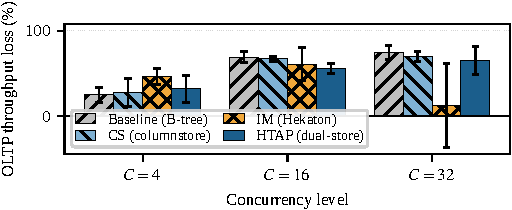
\includegraphics[width=\columnwidth]{figures/fig3_degradation.pdf}
\caption{OLTP throughput loss when the workload mix changes from 80/20 to
50/50, per configuration and concurrency level (mean $\pm$ standard
deviation).}
\label{fig:degradation}
\end{figure}

\subsection{Interference Under Mixed Workloads}
At $C = 16$, moving from the 80/20 to the 50/50 mix costs CS
67.4\,\%\,$\pm$\,2.8\,\% of its transactional throughput against
55.9\,\%\,$\pm$\,6.3\,\% for the hybrid configuration; the 11.5
percentage-point difference is significant with a large effect
($p < 0.001$, $d = 2.32$).
Fig.~\ref{fig:degradation} shows the advantage to be concurrency-dependent:
at $C = 4$ all configurations lose between 25\,\% and 46\,\% with no
significant CS--HTAP difference, and at $C = 32$ the comparison is dominated
by the variance of IM, whose 80/20 throughput is itself depressed by
row-mode analytical scans. The isolation mechanism is explicit: in CS,
batch-mode scans share the buffer pool and CPU threads with OLTP statements
on the same disk-based schema, whereas in the dual-store layout analytical
queries read the \texttt{cs} columnstore while transactions operate on
memory-optimized tables that never touch the buffer pool. Losing 67.4\,\% of
transactional capacity is critical under a service-level agreement, and the
magnitude agrees with the 50--70\,\% range reported for disk-based
systems~\cite{wu2025}.

\subsection{Regression Analysis}
Two OLS models with log-transformed dependent variables quantify each
factor's contribution (Table~\ref{tab:ols}), with Baseline and the 80/20 mix
as reference categories. The HTAP coefficient of $+1.965$ corresponds to
$e^{1.965} \approx 7.1\times$ the transactional throughput of Baseline,
while $-1.382$ in the latency model corresponds to a
$e^{1.382} \approx 4.0\times$ reduction of analytical latency. The CS
coefficient in the throughput model is not significant ($p = 0.600$): adding
a columnstore index alone does not improve transactional throughput.

\begin{table}[t]
\caption{OLS regression coefficients ($N = 1\,065$)}
\label{tab:ols}
\centering
\footnotesize
\begin{tabular}{@{}lrrrr@{}}
\toprule
& \multicolumn{2}{c}{$\log(\text{OLTP thr.})$} & \multicolumn{2}{c}{$\log(\text{OLAP } P_{50})$}\\
\cmidrule(lr){2-3}\cmidrule(l){4-5}
\textbf{Parameter} & Coef. & $p$ & Coef. & $p$\\
\midrule
CS vs. Baseline        & $+0.021$ & 0.600  & $-0.636$ & $<0.001$\\
IM vs. Baseline        & $+0.708$ & $<0.001$ & $-1.166$ & $<0.001$\\
HTAP vs. Baseline      & $+1.965$ & $<0.001$ & $-1.382$ & $<0.001$\\
Mix 50/50 vs. 80/20    & $-0.821$ & $<0.001$ & $+0.403$ & $<0.001$\\
Mix 20/80 vs. 80/20    & $-2.211$ & $<0.001$ & $+0.640$ & $<0.001$\\
$\log(\text{concurrency})$ & $+0.325$ & $<0.001$ & $+0.395$ & $<0.001$\\
\midrule
$R^2$ & \multicolumn{2}{c}{0.881} & \multicolumn{2}{c}{0.854}\\
\bottomrule
\end{tabular}
\end{table}

% =====================================================================
\section{Discussion}
% =====================================================================
The measurements expose a mechanism not quantified independently before: the
columnstore layer does not merely accelerate analytical queries, it also
\emph{indirectly protects transactional resources}. That is why the
dual-store configuration outperforms not only the disk-based configurations
but also IM, on the same Hekaton engine. In IM, analytical queries scan memory-optimized tables in row mode,
spending far more CPU cycles per row and saturating the processor at
$C = 16$ and $C = 32$; in the dual-store layout they are served in batch mode
from the columnstore copy, so transactions never compete for CPU. Accelerating analytics is therefore also a means of protecting OLTP
throughput --- a lever complementing the isolation-first perspective
of~\cite{kang2023} and the decoupled architectures of~\cite{huang2020,
yang2020}, here without network latency.

The practical rule is simple: when the workload mixes transactions and
analytics the dual-store layout is preferable at any ratio, while CS remains
the choice for purely analytical workloads and for servers lacking the memory
or the edition for In-Memory OLTP. Its preconditions are substantial: roughly
twice the memory, the cost of synchronizing the layers, and tolerance for
analytics over data that is not fresh.

\section{Threats to Validity}
\label{sec:threats}
Four limitations bound these results. First, and most importantly, the
evaluated dual-store configuration separates the two layers but runs no
synchronization mechanism (change data capture, replication or compaction),
whereas production systems pay that cost
continuously~\cite{huang2020, yang2020}; the reported gains are therefore an upper
bound at zero synchronization cost, quantifying how much interference
physical separation removes rather than the net benefit of a consistent
system. Second, the memory-optimized configurations use
\texttt{DURABILITY = SCHEMA\_ONLY} and read from RAM while the disk-based ones
read from an NVMe SSD, so comparisons across media mix the effect of
architecture with that of the medium; the cleanest are those within one
medium (HTAP vs. IM, CS vs. the HTAP analytical layer). Third, the \texttt{MAXDOP} asymmetry the engines require confounds the
HTAP--IM comparison, and its contribution was not isolated.
Fourth, the CPU-saturation explanation is derived from the query execution
model rather than direct profiling, and all measurements come from one
instance and dataset, so generalization requires caution.

% =====================================================================
\section{Conclusion}
% =====================================================================
Across 1\,070 valid runs over a 19.2-million-row real dataset, the dual-store
configuration of SQL Server 2022 dominated every tested mixed-workload
scenario, reaching 21\,920 ops/s at $C = 32$ --- 4.6$\times$ the in-memory
configuration and 9.0$\times$ the baseline --- at the lowest analytical
latency ($P_{50} = 924$\,ms under 80/20). The purely in-memory
configuration proved unexpectedly weak under mixed load despite the same
transactional engine, because row-mode analytical scans saturate the CPU,
while the disk-based columnstore configuration lost two thirds of its
transactional capacity once analytical load was added. That protective
effect, worth a factor of 3.3--6.9 here, deserves attention when HTAP systems
are tuned. Future work will measure the cost of continuous synchronization
and add direct CPU profiling.

\section*{Acknowledgment}
This work was carried out as a project for the Database Optimization course
in the Software Engineering master's program at the Polytechnic Faculty,
University of Zenica.

\balance

% =====================================================================
\bibliographystyle{IEEEtran}
\bibliography{refs_htap}

\end{document}
